\section{实时流体仿真系统的实现}
    本文的主要目标是基于WebGPU构建一个轻量级在线实时流体流体仿真系统。前文从物理模拟与流体渲染两个方面详细阐述了仿真系统的理论基础,本章将简要介绍WebGPU架构模型与API特性开始,并在此基础上进一步讨论流体模拟与渲染系统的具体实现,最后,本章使用流体仿真系统搭建了多个模拟场景,其实验结果全面体现了本文算法在轻量化、高效性与稳定性方面的优势,以及WebGPU广阔的应用场景。

    \begin{figure}[htbp]
    	\centering
    	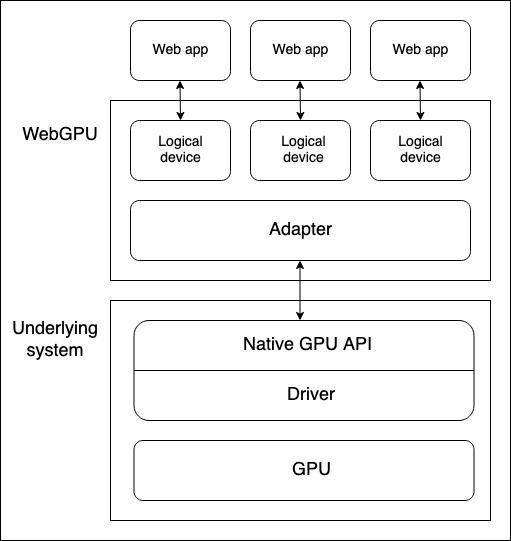
\includegraphics[width=.5\textwidth]{figures/webgpu/architecture.png}
    	\caption{WebGPU架构}
    \end{figure}

\subsection{WebGPU}
    WebGPU是一个全新的浏览器端图形API,它使开发人员能够使用底层系统的图形处理器(GPU)进行高性能计算并绘制可在浏览器中渲染的复杂图形。2023年5月,Chrome浏览器发布113版本,在稳定版中正式加入对WebGPU的支持。

    WebGPU并不是第一个浏览器图形API,2011年出现的WebGL是首个允许web页面直接将渲染计算传递给设备的GPU的图形接口。WebGL基于OpenGL设计实现,而自其发布之后,在原生平台又出现了新一代GPU API——微软的Direct3D 12、苹果的Metal以及Khronos组织的Vulkan,它们提供了大量新特性、更科学的设计与更高效的实现。这使得OpenGL逐渐落后于时代,同样WebGL也难以满足日新月异的浏览器应用的图形需求。因此,WebGPU应运而生,作为WebGL的继任者,它为现代GPU提供了更好的兼容性、支持更通用的GPU计算、更快的操作以及能够访问到更高级的GPU特性。
    
    WebGPU的设计更类似于Vulkan这类新一代GPU,摒弃了OpenGL全局状态机的管理模式。在与GPU交互时,WebGPU会先将所有指令都存储在指令队列(Commad Queue)中,一次性提交给GPU。一方面减少了CPU与GPU的通信损耗,另一方面在指令队列录制完毕后还可以多次使用,减少CPU冗余计算。最重要的WebGPU指令是设置绑定组(Bind Group)与管线(Pipeline)。绑定组描述了GPU计算时使用的存储资源的结构信息,而管线则确定了GPU如何计算,需要执行哪些着色器代码。后文将进一步介绍WebGPU支持的存储结构与管线配置。

    \begin{figure}
    	\centering
    	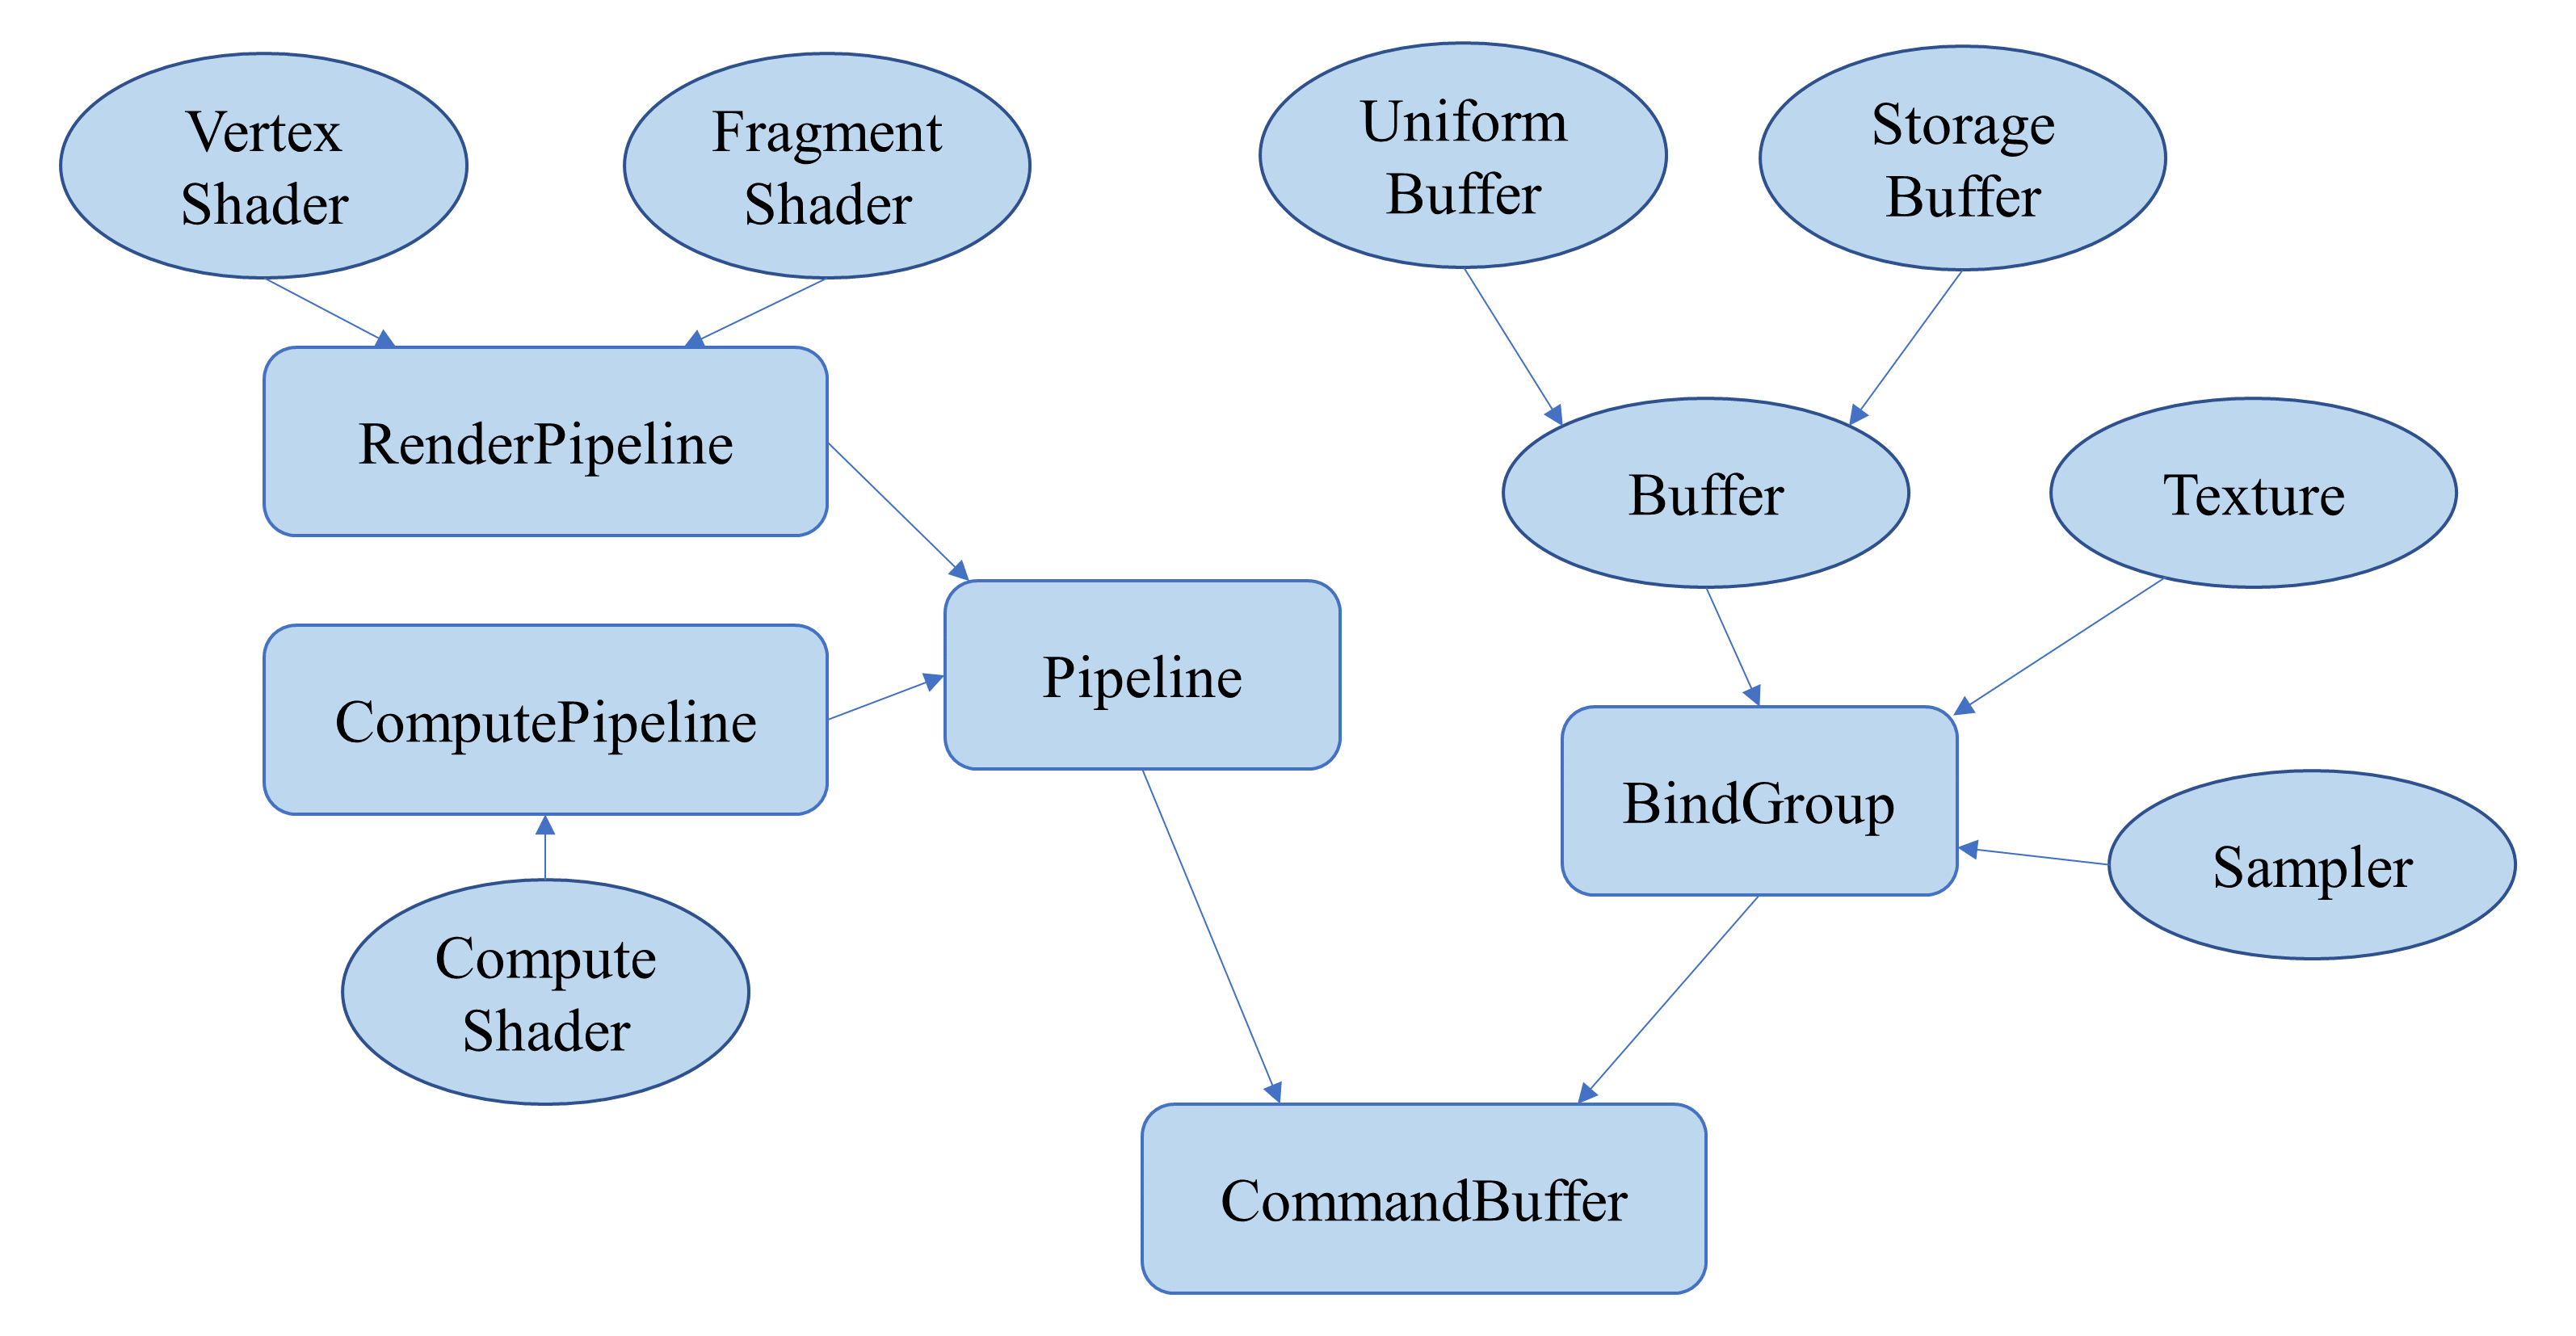
\includegraphics[width=.75\textwidth]{figures/webgpu/api.png}
    	\caption{WebGPU API结构}
    \end{figure}

\subsubsection{存储结构}
    WebGPU支持的存储类型有两种,Buffer与Texture。这两种存储结构以及采样器(Sampler)可以任意组合打包为绑定组,供计算管线与渲染管线使用。
    
    Buffer在存储中是线性结构,存储灵活自由。具体格式又分为两种:Uniform Buffer和Storage Buffer。其中Uniform Buffer是只读的,将数据传递到GPU后不可更改,在硬件上存储在常量内存区(Constant Memory),访问延迟较低。并且Uniform Buffer内存排布较为紧凑,需要以8字节为一块进行内存对齐,其空间最大为64KB。而Storage Buffer直接存储在显存上,可用空间非常大,但访问延迟也很高。
    
    基于以上特点,Uniform Buffer一般存储一些占用空间较小的,需要经常从CPU拷贝到GPU的常量信息,比如相机参数、光照信息、仿真参数、管线控制信息等。而Storage Buffer一般存储大量的,仅用于GPU计算的信息,比如仿真系统中每个粒子的物理量、空间网格结构、边界条件的体积贴图等。
    
    与Buffer不同,Texture在存储中是具有空间结构的,WebGPU支持1D/2D/3D纹理。在硬件结构上,Texture一般存储在专用的纹理内存中,访问速度较高,并且支持硬件的纹理采样、颜色空间转换等功能。另外,Texture对存储的数据结构有严格的要求,在创建时需要用户显示指定,比如rgba8unorm-srgb,意为4通道8位的纹理,其取值范围位0到1,并且数据精度为0-1均匀划分,另外在数据存储或读取时会自动做SRGB与线性之间的颜色空间转换。显然,Texture只用于纹理数据,或渲染管线输出的渲染目标(Render Target),例如流体渲染光栅化阶段的深度图与厚度图。

\subsubsection{管线}
    WebGPU管线分为两种,一个是传统的渲染管线(Render Pipeline),也就是GPU最基础的光栅化管线,另一个是计算管线(Compute Pipeline),它是WebGPU相对于WebGL引入的最重要新特性之一,它给开发者开放了GPU的通用计算能力,我们的流体仿真系统中绝大部分并行计算都依赖WebGPU计算管线实现。
    
    WebGPU渲染管线分为两个阶段(Stage),分别是顶点阶段和片元阶段,这两个阶段可以由开发者编写着色器程序进行自由控制。相比于其他现代图形API,WebGPU并不支持一些新型着色器,比如Tessellation Shader、Geometry Shader和Mesh Shader。这些着色器对应的阶段如顶点装配、光栅化、深度模板测试等直接由固定的硬件程序执行,开发者可以在管线创建时进行一些可选项的配置,比如图元拓扑结构、三角形剔除模式、alpha混合等。在仿真系统中,流体粒子的光栅化、流体屏幕空间渲染都使用渲染管线实现。
    
    WebGPU计算管线赋予了开发者极大的自由度,我们可以在计算着色器中读取Buffer或Texture中的数据,完成计算后将结果写入灵活的Storage Buffer中。在执行计算管线时可以指定任意数量个工作组(Work Group),并且工作组中的并行线程数量也可以在计算着色器中指定。并行计算往往会涉及到数据一致性的问题,WebGPU支持对同一存储空间进行原子读写操作,另外,同一工作组内的线程也可以在代码执行的任意位置进行线程同步。例如,在将数据读取到共享内存后,往往需要进行一次线程同步,以保证不同线程读取的数据均完成后再进行后续的计算操作。

\subsection{物理模拟系统}
    本文的目标是构建一个实时流体仿真系统,第三四五章分别介绍了流体模拟中的压强求解算法、非压强力算法与近邻粒子搜索算法。这些算法均具有高度的并行性,可以充分利用GPU算力优势。算法1给出了本系统的伪代码,其中所有for循环都是使用WebGPU的计算管线并行实现的,且每个for循环均对应一个计算着色器。由于本算法完全使用GPU并行化,所以不需要CPU与GPU之间的数据通信,这大大提高了计算效率。
    
    另外,本文也充分考虑了存储空间的优化。一个时间步之内,每个计算管线使用到的物理量不同,其中一些是完全互斥的,那么它们就可以重复使用同一块存储空间,比如在计算法向 $\mathbf n_i$ 时可以占用粒子位置 $\mathbf x_i^*$ 的存储空间。最终,在不影响数据对齐的前提下,每个粒子相关的物理量所占用的空间仅为84字节(32位浮点数精度)。

    \begin{algorithm}
    	\caption{流体仿真}
    	\begin{algorithmic}[1]
     
    	\ForAll{ particles $i$ } \Comment{ semi-implicit time integration }
    		\State apply force $\mathbf v_i \leftarrow \mathbf v_i + \Delta t \mathbf \, a_i$
    		\State predict position $\mathbf x^*_i \leftarrow  \mathbf x_i + \Delta t \mathbf \, v_i$
    	\EndFor

    	\ForAll{ particles $i$ } \Comment{ neighborhood particle search }
    		\State insert $\mathbf x^*_i$ into grid cell
    	\EndFor
    	\State calculate prefix sum of gridCellParticleCounts.
    	\ForAll{ particles $i$ } 
    		\State get sorted index of $\mathbf x^*_i$ \quad \Comment{ counting sort }
    	\EndFor
    	\ForAll{ particles $i$ } 
    		\State calculate count of neighboring particles of $\mathbf x^*_i$
    	\EndFor
    	\State calculate prefix sum of neighborParticleCounts.
    	\ForAll{ all particles $i$ } 
    		\State find neighboring particles $N_i(\mathbf x^*_i)$
    	\EndFor

    	\While { iter < iterCount } \Comment{ solve pressure constrain }
    		\ForAll{ particles $i$ }
    			\State calculate boundary volume $V_i^{\mathcal B}$ and boundary point $\mathbf x_i^*$  \quad \Comment{ Eq.\,3.15 }
    		\EndFor
    		\ForAll{ particles $i$ }
    			\State calculate $\lambda_i$  \quad \Comment{ Eqs.\,3.10,\,3.17 }
    		\EndFor
    		\ForAll{ particles $i$ }
    			\State calculate $\Delta \mathbf x_i$  \quad \Comment{ Eqs.\,3.12,\,3.19 }
    		\EndFor
    		\ForAll{ particles $i$ }
    			\State update predicted position $\mathbf x^*_i \leftarrow \mathbf x^*_i + \Delta \mathbf x_i$
    		\EndFor
    	\EndWhile
    	\ForAll{ particles $i$ }
    		\State update velocity $\mathbf v_i \leftarrow \frac{1}{\Delta t} (\mathbf x^*_i -\mathbf x_i)$
    		\State update position $\mathbf x_i \leftarrow \mathbf x^*_i$
    		\State update density $\rho_i = \sum_j m_j W_{ij}$
    	\EndFor

        \ForAll{ particles $i$ } \Comment{ apply non pressure forces }
            \State calculate normal $\mathbf n_i$  \quad \Comment{ Eq.\,4.4 }
            \State calculate vorticity $\omega_i$  \quad \Comment{ Eq.\,4.7 }
        \EndFor
        \ForAll{ particles $i$ }
            \State apply surface tension, vorticity confinement and XSPH \Comment{ Eqs.\,4.5,\,4.6,\,4.8 }
            \State calculate acceleration $\mathbf a_i \leftarrow \frac{\mathbf F_i}{m_i}$
        \EndFor
     
        \end{algorithmic}
    \end{algorithm}

\subsection{渲染系统}
    在实现了流体模拟系统之后,渲染系统需要将其实时渲染出来。本文第六章介绍了屏幕空间流体渲染算法,在WebGPU实现中,本文采用了渲染-计算-渲染的混合架构。首先使用两个渲染管线,借助硬件高效光栅化大量流体粒子,得到深度图和厚度图。然后使用两个计算管线,分别对深度图进行X方向和Y方向的窄域滤波。最后再使用一个渲染管线完成着色并输出到屏幕上。

    \begin{figure}
    	\centering
    	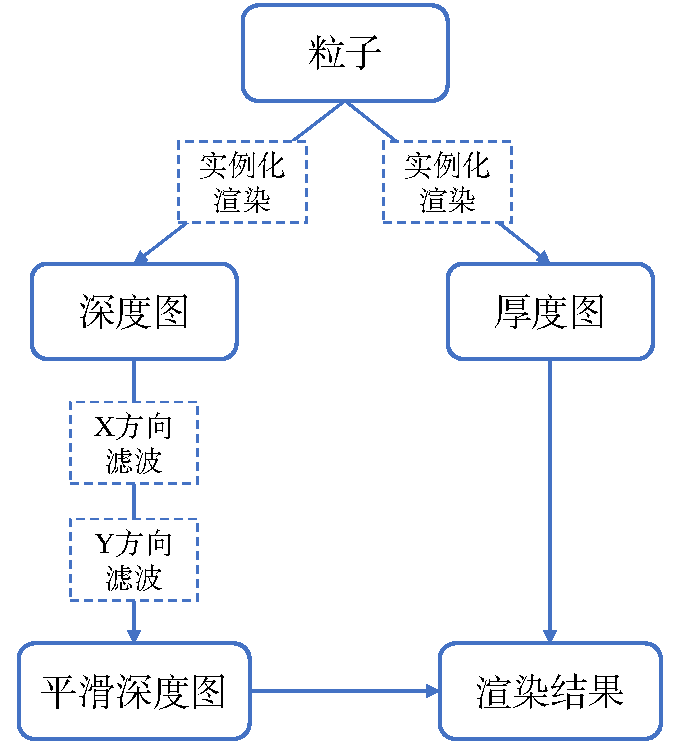
\includegraphics[width=.45\textwidth]{figures/webgpu/pipeline.pdf}
    	\caption{屏幕空间流体渲染流程图}
    \end{figure}

\subsection{实际仿真场景与性能分析}
    在本文搭建的流体仿真系统中,可人为调整的参数设置如下:仿真时间步长 $\Delta t = 0.005s$,密度约束中的松弛因子 $\varepsilon = 10^{-6}$,密度约束迭代次数为5次,表面张力 $\alpha = 0.5$,人工粘性 $\beta=0.01$,涡量补偿$\gamma = 0.1$。

    \begin{table}
    	\centering
    	\caption{帧率对比}
    	\begin{tabular}{ccc}
    	\toprule
    	实验场景 & 粒子数量(个) & 平均帧率(FPS) \\
    	\midrule
    	体素化兔子 & 32522	& 58.18	\\
    	立方体 & 68921	& 33.94	\\
    	水滴	 & 44489 & 45.07	\\
    	双溃坝 & 56448	& 27.08	\\
    	圆环边界 & 68921	& 22.88	\\
    	\bottomrule
    	\end{tabular}
    \end{table}
    
    \begin{table}
    	\centering
    	\caption{计算耗时对比}
    	\begin{tabular}{ccccccccc}
    	\toprule
    	\multirow{2}{*}{实验场景} &
    	\multicolumn{4}{c}{模拟} &
    	\multicolumn{4}{c}{渲染} \\
    	\cmidrule(lr){2-5} \cmidrule(lr){6-9}
    	& 时间积分 & 邻域查找 & 压强约束 & 非压强力 & 粒子光栅化 & 深度平滑 & 流体渲染 & 其他 \\
    	\midrule
    	体素化兔子
    	& 0.072	& 4.378	& 5.511	& 2.178	& 1.532	& 1.331	& 0.791	& 0.551	\\
    	立方体坠落
    	& 0.121	& 9.426	& 12.426& 4.871	& 2.718 & 1.364 & 0.848	& 0.547	\\
    	水滴			
    	& 0.094 & 5.822 & 8.092	& 3.451	& 2.034	& 1.385	& 0.742	& 0.578	\\
    	双溃坝		
    	& 0.104	& 12.070& 15.154& 6.077	& 3.117	& 1.697	& 0.989	& 0.672	\\
    	圆环边界		
    	& 0.121	& 14.949& 20.394& 7.452	& 3.808	& 1.780	& 1.080	& 0.707 \\
    	\bottomrule
    	\multicolumn{9}{r}{单位:毫秒}\\
    	\end{tabular}
    	\label{tab:comp}
    \end{table}
    
    图\ref{fig:result}展示了本仿真系统在五种不同实现场景下的模拟与渲染结果,从左到右分别是:体素化兔子、立方体、水滴、双溃坝与圆环边界,从上到下则表示了随着时间推移流体坠落的效果。其中兔子场景展示了本系统体素化控制流体初始边界的能力,水滴坠落展示了生动的流体表面张力效果,圆环边界展示了流体与固体交互的效果,立方体坠落与双溃坝则展示了本系统应对较大规模流体粒子的仿真效果。这五种复杂场景全面地体现了本系统的稳定性与模拟渲染的真实感。

    \begin{figure}
    	\centering
    	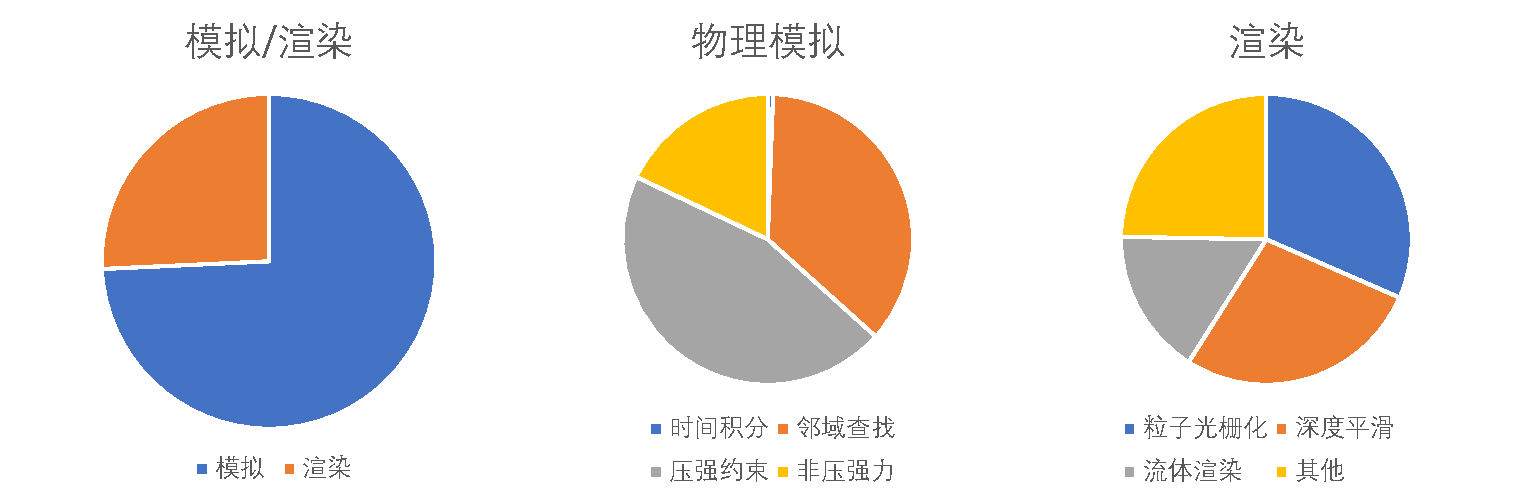
\includegraphics[width=0.9\textwidth]{figures/webgpu/comp.pdf}
    	\caption{计算耗时对比}
    	\label{fig:comp}
    \end{figure}
    
    \begin{figure}
    	\centering
    	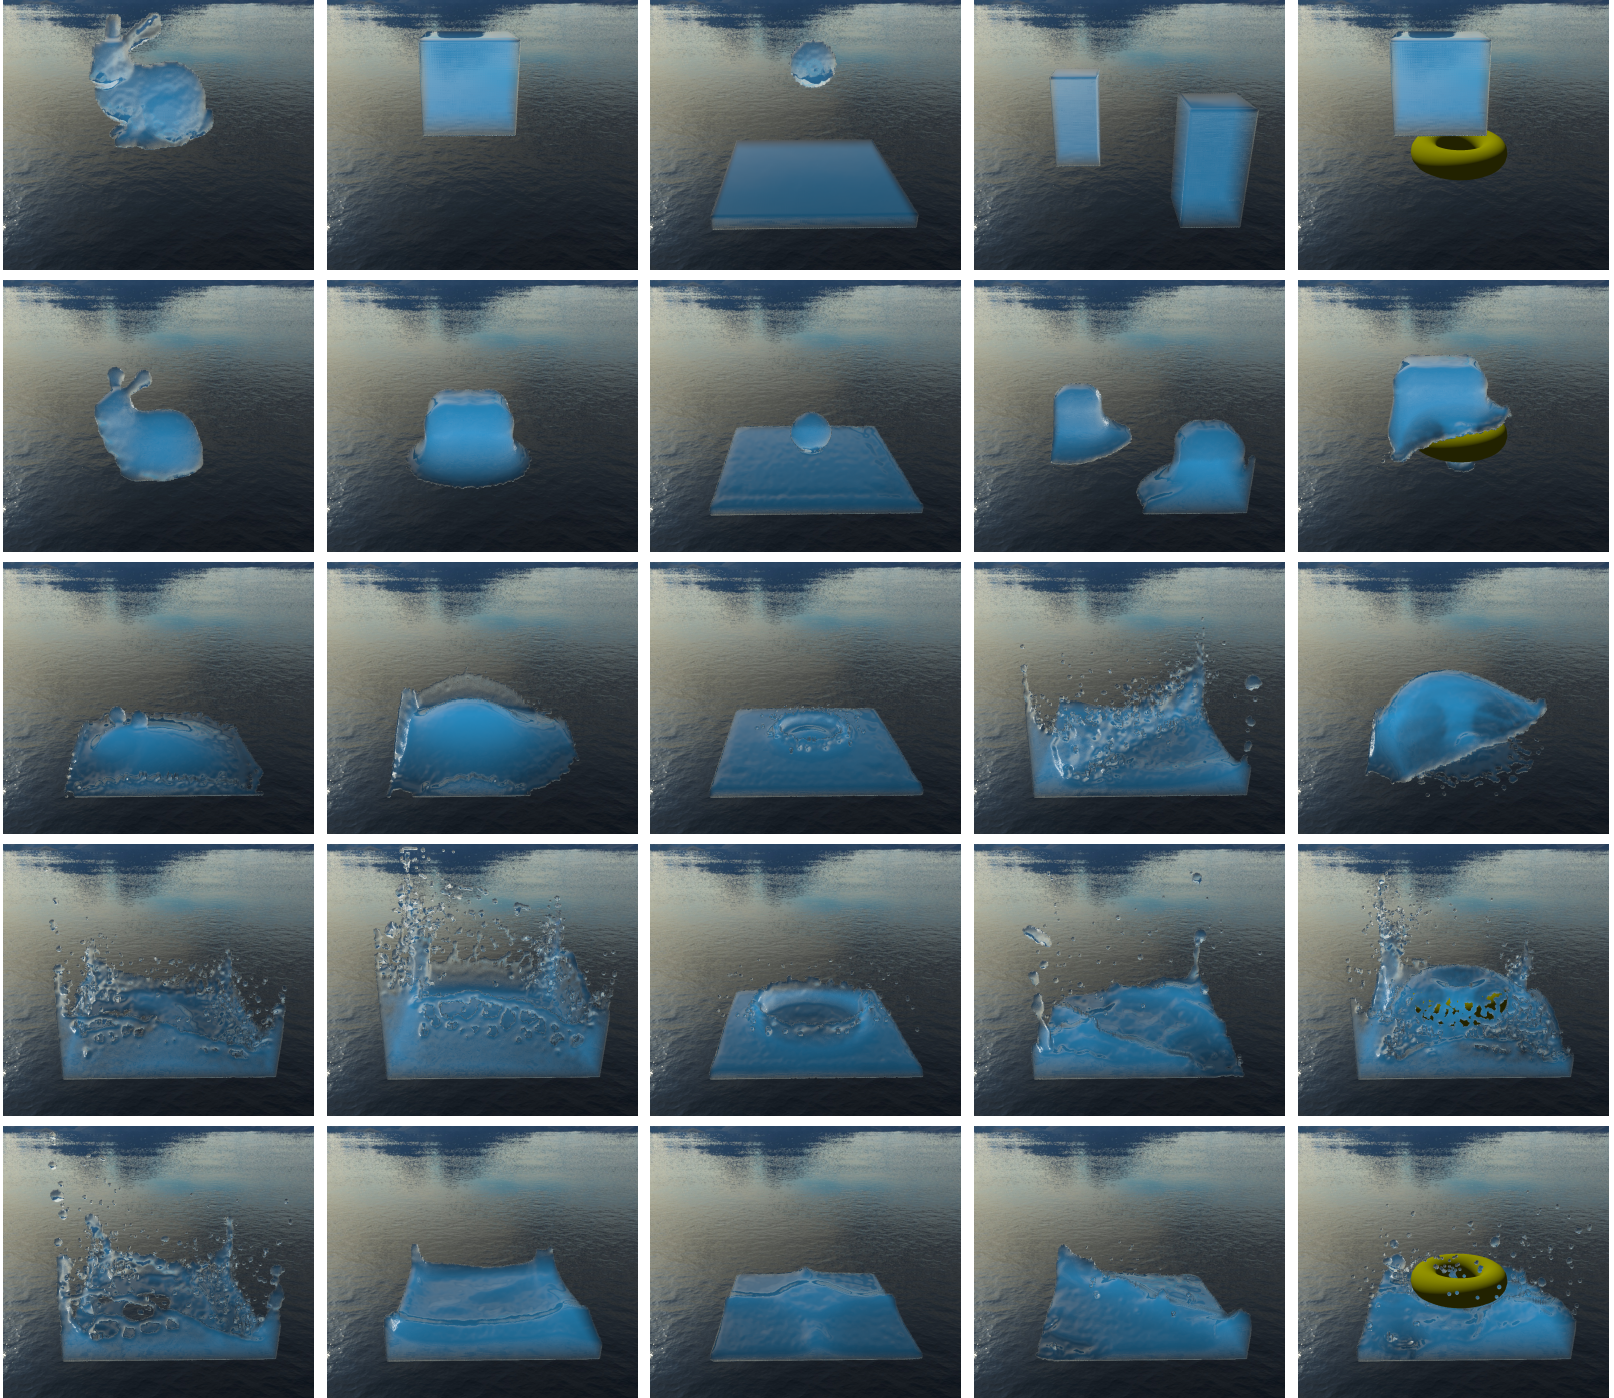
\includegraphics[width=0.99\textwidth]{figures/webgpu/demo.png}
    	\caption{实验结果(仿真场景:体素化兔子、立方体坠落、水滴、双溃坝与圆环边界)}
    	\label{fig:result}
    \end{figure}
    
    本章实验场景的测试平台硬件规格是:CPU为Intel Core i5-1135G7,RAM为16G,GPU为Intel Iris Xe(80EU)。本仿真系统仅运行在性能孱弱的集成显卡上,但仍然能够实时仿真并达到较流畅的30FPS,由此可见本文提出的轻量化流体仿真系统的高效性能。
    
    表\ref{tab:comp}与图\ref{fig:comp}给出了五个仿真场景前300帧每个模块计算的平均耗时。可以看出物理模拟计算耗时占每帧耗时的3/4,而这其中邻域粒子查找与压强约束求解又占了绝大部分时间。这点符合预期,因为邻域粒子查找数据相关性较强,其并行化算法较复杂,而压强约束需要迭代求解一个大型非线性系统,是整个仿真系统最耗时的计算模块。另外,由于我们将三种非压强力的实现压缩到了两个计算着色器中,这使得非压强力的计算耗时大大减少,远小于压强求解。在渲染计算方面,深度图的平滑是复杂度最高的计算过程,每个像素都需要采样大量相邻像素进行滤波计算,但由于我们在具体实现中使用了工作组线程间的共享缓存,大大减少了访存周期,使得深度平滑计算与硬件光栅化计算的耗时平分秋色。

\subsection{本章小结}
    本章阐述了实时流体仿真系统的实现。首先,本章从管线个存储结构两方面介绍了WebGPU的API架构,以及每种API在仿真系统的哪些模块中被使用到。其次,本章分别通过物理模拟模块的算法伪代码与流体渲染模块的流程图介绍了如何使用WebGPU实现仿真系统。最后,本章通过五个复杂场景证明了算法的稳定性与高效性,在核显平台仍然能达到实时仿真的帧率。总的来说,本文实现的流体仿真系统在实际应用中具有广阔的前景,可用于网页游戏、影视特效和虚拟现实等领域,提供更真实的交互和沉浸式体验。